\chapter{Аналитический раздел}

\section{Постановка задачи}
Необходимо разработать программу для отслеживания состояния склада с автозапчастями. В частности требуется хранить информацию о том, какой пользователь положил деталь на склад и какой ее забрал.

Некоторые запчасти можно заменить на подобные им от другого производителя, поэтому у пользователя должна быть возможность поиска на складе не только самой детали, но и ее аналогов.

\section{Формализация данных}\label{sec:formalisation}
База данных должна содержать информацию о:
\begin{itemize}
	\item деталях для автомобилей;
	\item производителях автозапчастей;
	\item текущем состоянии склада и истории его изменения;
	\item пользователях системы.
\end{itemize}

Информация о детали должна содержать:
\begin{itemize}
	\item артикул;
	\item название на русском и английском языках;
	\item возможные варианты замены;
	\item идентификатор производителя.
\end{itemize}

Производитель автозапчасти характеризуется страной и названием.

Пользователь характеризуется следующими параметрами:
\begin{itemize}
	\item Личные данные: имя, фамилия, дата рождения;
	\item уровень доступа к системе;
	\item данными авторизации: логин, пароль.
\end{itemize}

\section{Типы пользователей}
В системе должно быть разделение пользователей по уровню доступа к информации и возможностям ее изменения. Каждый пользователь должен авторизоваться прежде чем начать работу с приложением. Уровни доступа различных пользователей представлены на таблице \ref{table:1}

\begin{table}[H]
	\caption{Уровни доступа различных пользователей}
	\label{table:1}
	\begin{tabular}{|l|l|}
		\hline
		\textbf{Тип пользователя} & \textbf{Функционал}                                                                                                                                                                                      \\ \hline
		Неавторизованный          & Регистрация, авторизация                                                                                                                                                                                 \\ \hline
		Клиент                    & Просматривать наличие запчастей на складе                                                                                                                                                                \\ \hline
		Кладовщик                 & Добавлять запчасти на склад                                                                                                                                                                              \\ \hline
		Продавец                  & Забирать запчасти со склада                                                                                                                                                                              \\ \hline
		Администратор             & \begin{tabular}[c]{@{}l@{}}Изменять уровни привилегий других пользователей,\\ модифицировать информацию о запчастях, \\ производителях и заменах, просматривать\\ историю изменения склада.\end{tabular} \\ \hline
	\end{tabular}
\end{table}

Диаграмма вариантов использования представлена на рисунке \ref{img:usecase-diagram}.
\begin{center}
	\begin{figure}[H]
		\centering
		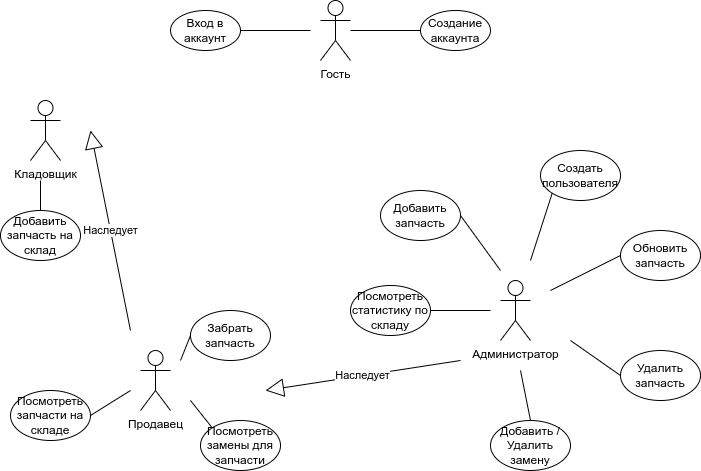
\includegraphics[scale=0.5]{inc/img/use-case.png}
		\caption{Диаграмма вариантов использования}
		\label{img:usecase-diagram}
	\end{figure}
\end{center}

Диаграмма сущностей в нотации Чена представлена на рисунке \ref{img:er-diargram}
\begin{center}
	\begin{figure}[H]
		\centering
		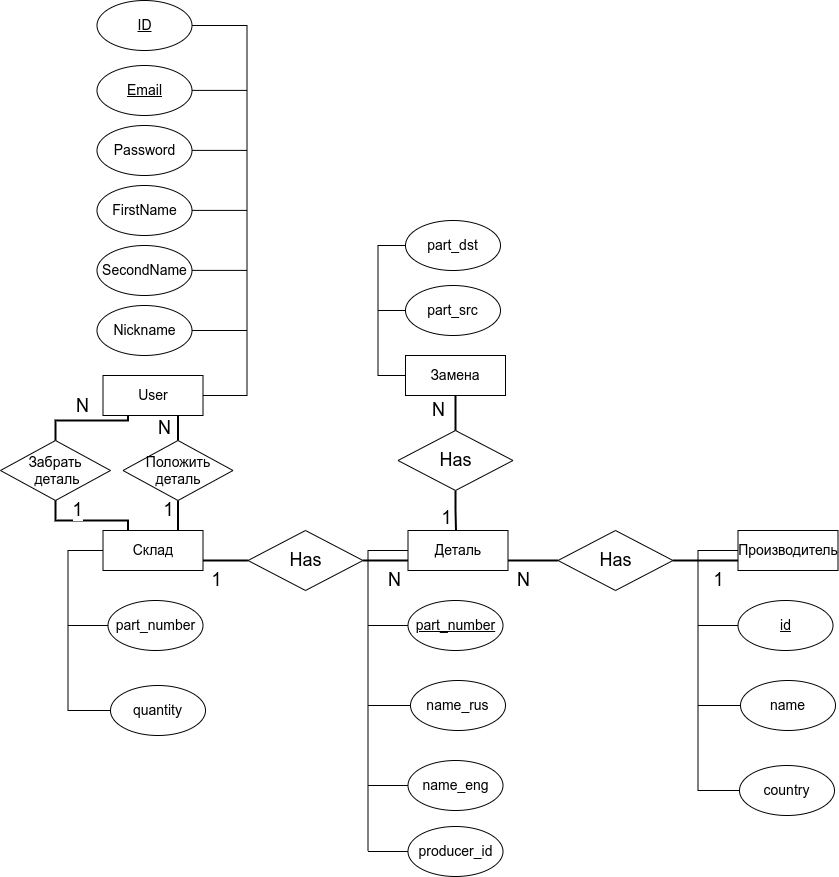
\includegraphics[scale=0.5]{inc/img/er-diagram.png}
		\caption{Диаграмма сущностей в нотации Чена }
		\label{img:er-diargram}
	\end{figure}
\end{center}

\section{Модели хранения данных}

Модели данных — вероятно, важнейшая часть разработки программного обеспечения в силу оказываемого ими глубочайшего воздействия не только на процесс
разработки, но и на наше представление о решаемой проблеме \cite{kleppman}.
Можно выделить три основных модели хранения данных:
\begin{itemize}
	\item иерархическая;
	\item сетевая;
	\item реляционная.
\end{itemize}

\textbf{Иерархическая модель}
В иерархической модели данных используется представление базы данных в виде древовидной структуры, состоящей из объектов различных уровней. Между объектами существуют связи, каждый объект может включать в себя несколько объектов более низкого уровня. Такие объекты находятся в отношении предка к потомку, при этом возможна ситуация, когда объект-предок имеет несколько потомков, тогда как у объекта-потомка обязателен только один предок.

\textbf{Сетевая модель}
В древовидной структуре последней у каждой записи была ровно одна родительская запись. В сетевой же у каждой записи могло быть несколько родительских. Например, в базе
может быть одна запись с названием города со ссылкой на нее
для каждого живущего там пользователя. В сетевой модели появилась возможность моделировать связи «многие-к-одному» и «многие-ко-многим».

Главным недостатком сетевой модели данных являются жесткость и высокая сложность схемы базы данных, построенной на основе этой модели. Так как логика процедуры выбора данных зависит от физической организации этих данных, то эта модель не является полностью независимой от приложения. Иначе говоря, если будет необходимо изменить структуру данных, то нужно будет изменять и приложение.

\textbf{Реляционная модель}
Реляционная модель состоит из набора двумерных таблиц. При табличной организации отсутствует иерархия элементов. Таблицы состоят из строк – записей и столбцов – полей. На пересечении строк и столбцов находятся конкретные значения. Для каждого поля определяется множество его значений. За счет возможности просмотра строк и столбцов в любом порядке достигается гибкость выбора подмножества элементов.

В реляционной базе данных оптимизатор запросов автоматически принимает решение о том, в каком порядке выполнять части запроса и какие индексы использовать.

\textbf{Выбор модели хранения данных}
Все сущности системы имеют четкую структуру, которая не меняется от объекта к объекту, поэтому для хранения данных подойдет реляционная модель.

\section{Аутентификация пользователей в системе}

Аутентификацию пользователей в системе можно проводить с использованием спецификации OAuth1 \cite{oauth1}. Такой подход предполагает следующую последовательность:
\begin{itemize}
	\item пользователь отправляет запрос, в котором указывает свои логин и пароль;
	\item приложение ищет пользователя, с указанными параметрами в базе данных и, в случает успеха, возвращает токен, с использованием которого клиент может осуществлять последующие запросы.
\end{itemize}

В таком случае необходимо где-то хранить связь токена с идентификаторам пользователя, которому он принадлежит. Для таких целей подойдет In Memory ключ-значение СУБД, которая обеспечивает быстрый поиск за счет того, что все данные хранятся в оперативной памяти. Главной проблемой таких СУБД является возможность утери данных, к примеру, при отключении электропитания, что не является критичным для хранения токенов, так как пользователю будет достаточно еще раз заполнить форму с логином и паролем для восстановления сессии.

В качестве СУБД для хранения сессий авторизованных пользователей может подойти Redis \cite{redis}.
